%\documentclass[twoside,openright,a4paper,11pt]{book}
%
%
\usepackage[utf8]{inputenc}
\usepackage[francais]{babel}
\usepackage[T1]{fontenc}

\addto\captionsfrench{\def\tablename{\textsc{Tableau}}}% pour avoir TABLEAU et pas TABLE dans les légendes des tableaux

%%%%%%% MISE EN PAGES %%%%%%
\usepackage{geometry}
\geometry{outer=2cm,inner=3cm,top=3cm}

\setcounter{tocdepth}{3}     % Dans la table des matieres
\setcounter{secnumdepth}{3}  % Avec un numero.
\usepackage{setspace}

\usepackage{fancyhdr}	% marge en haut et en bas
\pagestyle{fancy}

\fancyhead{}	% vide l'entête
\fancyfoot{} % vide le pied~de~page

\fancyhead[RO]{\leftmark}
\fancyhead[LE]{\rightmark}
\fancyfoot[C]{\thepage}	% numéro de page en bas au centre

\renewcommand{\headrulewidth}{0.4pt} % épaisseur du trait en haut
\renewcommand{\footrulewidth}{0.4pt} % épaisseur du trait en bas

\fancypagestyle{mypagestyle}{%
    \fancyhead{}	
    \fancyfoot{} 
    \fancyfoot[C]{\thepage}
    \renewcommand{\headrulewidth}{0.4pt} 
	\renewcommand{\footrulewidth}{0.4pt} 
}

\fancypagestyle{couvertureAbstract}{%
    \fancyhead{}	
    \fancyfoot{} 
    \fancyfoot[C]{}
	\renewcommand{\headrulewidth}{0pt} 
	\renewcommand{\footrulewidth}{0pt} 
}
%
\usepackage{layout}
\usepackage{tocbibind} % include tableofcontent in itself

%%%%%% PAGE DE GARDE %%%%%%

\geometry{outer=2cm,inner=3cm,top=3cm}
\usepackage[scaled]{helvet} % font used on cover (Helvetica)
\usepackage{eso-pic} % to set background picture
\usepackage{multicol} % for back cover (abstracts)
\usepackage{graphicx} % to include logos
\usepackage{tikz} % to compose background picture

% Colors (extracted from SPI's template)
\definecolor{boxcolor1}{rgb}{0.91373,0.92941,0.87451}
\definecolor{boxcolor2}{rgb}{0.94902,0.93333,0.91373}
\definecolor{boxcolor3}{rgb}{0.76078,0.87843,0.17647}
\definecolor{headercolor}{rgb}{0.94118,0.30980,0.17255}
\definecolor{namecolor}{rgb}{1.0,0.4,0.0}
\definecolor{titlecolor}{rgb}{0.19216,0.51765,0.60784}
% Also used: gray, teal (predefined by xcolor package, usually loaded by document class)

% Cover environment, to keep changes local
\newenvironment{cover}{%
  \fontfamily{phv}\selectfont % Select Helvetica font
  \pagestyle{empty} % No page number
}{
  \addtocounter{page}{-1}
  \cleardoublepage
}

% Macro for background common to front and back
\newcommand{\tikzBG}{%
  \path (0,0) rectangle (1,1);
  %TODO: You should adjust the bottom height of the following rectangle to fit your abstract's length
  \path [fill=boxcolor1] (.0571,.11) rectangle (.481,.963); 
  \path [fill=boxcolor2] (.4333,.697) rectangle (.9048,.7475);
  \path [fill=boxcolor2] (.4333,.7811) rectangle (.9048,.8316);
  \path [fill=boxcolor2] (.4333,.8687) rectangle (.9048,.9192);
  \path [fill=boxcolor3] (.0571,.7879) rectangle (.5762,.8316);
  \node[inner sep=0pt] at (0.2285,0.8788) [above left] {%
    
\includegraphics[height=.0707\paperheight,keepaspectratio]{./figures/logo/logo_unb.png}};
  \node[inner sep=0pt] at (0.6667,0.8788) [above right] {%
    
\includegraphics[height=.0808\paperheight,keepaspectratio]{./figures/logo/logo_ecn_color.png}};
  \node at (.0571,.8316) [above right,color=headercolor] {%
    \fontsize{29}{35}\selectfont\bfseries Th\`ese de Doctorat};
}

% Macro for repeated information (to avoid insconsistency)
%TODO: fill in with no formatting but desired case
\newcommand{\firstName}{Jean-Rémy}
\newcommand{\surname}{Gloaguen}
\newcommand{\thesisTitle}{Estimation du niveau sonore de sources d'intérêts au sein de mixtures sonores urbaines : application au trafic routier}

%%%%%%% SYMBOLES %%%%%
\usepackage{tipa}	% pour avoir l'accent concave
\usepackage{lmodern}	% pour les guillemets
\usepackage{gensymb}	% pour les degrés
\usepackage{enumitem}	% pour changer le symbole de l'item (\begin{itemize}[label=$\bullet$])

%%%%%%% EQUATION %%%%%%
\usepackage{amssymb}
\usepackage{amsmath}
\usepackage{fancybox}
\usepackage{xfrac}	% fraction de type "1/4"
\usepackage{cases}	% système équation
\usepackage[overload]{empheq}
\usepackage{bm}		% pour mettre en gras .
\usepackage{units} 	% x/y barre latérale pour les fractions
%
%%%%%%% FIGURE %%%%%%
\usepackage{subfigure}	% utiliser subfigure
\usepackage{float}	% utiliser H dans les figures
%
%%%%%% TABLEAUX %%%%%%
\usepackage{array,multirow,makecell}
%\addto\captionsfrench{\def\tablename{\textsc{Tableau}}}% pour avoir TABLEAU et pas TABLE dans les légendes des tableaux
\usepackage{colortbl} % pour avoir des lignes colorées dans les tableau
%\usepackage{slashbox} % pour les \backslashbox
%\usepackage{subcaption}
\usepackage{hhline}	% pour les lignes horizontales 
\usepackage{tabularx} % permet itemize dans les cellules
\usepackage{booktabs}
\usepackage{longtable}	% pour les tableaux longs

\newcolumntype{L}[1]{>{\raggedright\let\newline\\\arraybackslash\hspace{0pt}}m{#1}}
\newcolumntype{C}[1]{>{\centering\let\newline\\\arraybackslash\hspace{0pt}}m{#1}}
\newcolumntype{R}[1]{>{\raggedleft\let\newline\\\arraybackslash\hspace{0pt}}m{#1}}

%%%%% ALGORITHME %%%%%
\usepackage{algorithm}
\usepackage{algorithmic}

%%%%% BIBLIO %%%%%
\usepackage[fixlanguage]{babelbib}
\selectbiblanguage{french}
\usepackage{breakcites}	% pour couper les références en bout de ligne

%%%%% APPENDICES %%%%%%%
\usepackage[toc,page]{appendix}

%%%%%%%%%%%%%%%%%%%%%
\usepackage{url}	% gérer les adresses www.
\linespread{1.2}	% interligne

\cleardoublepage
%
%\begin{document}

\chapter{Cartographie et mesures acoustiques}
\thispagestyle{empty}

\section{État de l'art en cartographie}
En 2016, au sein de l'Union Européenne (UE), plus de 70 $\%$ de la population vit dans des zones urbaines, incluant les centres-villes et les banlieues, soit quasiment 340 millions d'habitants \cite{europ-commission_data_2017}. Cette concentration soulève de grandes questions autour de l'organisation de l'espace urbain afin d'offrir une qualité de vie acceptable au citadin. En effet avec de telles densités (environ 3000 habitants au km$^2$) plusieurs formes de pollutions viennent dégrader l'environnement urbain. Des sources de désagrément perçu par le citadin, le bruit est le phénomène qui provoque le plus de gène après la pollution de l'air. \\

On estime, en Europe, que près de 200 millions de personnes sont exposées quotidiennement à des niveaux sonores supérieurs à 55 dB, soit 40$\%$ de la population. Près de 20 $\%$ atteignent même plus de 65 dB(A) en journée et plus de 30 $\%$ sont touchés par un niveau sonore excédant 55 dB(A) la nuit \cite{who_burden_2017}. De tel niveau sonore engendre chez près de 8 millions de personnes des troubles du sommeil mais aussi une détérioration de la santé de certain : on estime que le bruit est à l'origine de près de 900 000 cas d'hypertension, de 43 000 hospitalisations et de 10 000 cas de mort prématurés. C'est donc un enjeu majeur de santé public que l'UE doit traiter. De plus, si le bruit en ville impact les citadins, il ne faut pas oublier qu'il se fait également ressentir au delà dans les campagnes et qu'il impact aussi la faune sauvage \cite{dutilleux_anthropogenic_2012} en leur causant du stress ou en compliquant leur communication. \\

Si le bruit en ville provient en partie des activités humaines (conversation, musique provenant des bars ou des discothèques), la majeur partie du bruit est provoqué par l'activité du transport, qu'il soit routier, aérien ou  ferroviaire \cite{zannin_characterization_2013}. Ainsi, c'est en juin 2002 qu'est instaurée la directive européenne 2002/49/EC \cite{directive} dont le but de mieux connaitre la répartition du bruit en ville (et donc son impact sur les populations) en fonction des principales sources de bruit en ville (trafic routier, ferroviaire, aéroportuaire et  des Installations Classées pour la Protection de l'Environnement ICPE). Cette directive prévoit, dans les agglomérations de plus de 100 000 habitants, l'évaluation du niveau sonore de ces sources afin :

\begin{itemize}
	\item d'évaluer l'exposition au bruit des populations basée sur des méthodes communes aux pays européens,
	\item d'informer les populations sur leur niveau sonore d'exposition et sur les effets du bruit sur la santé,
	\item de connaitre et de délimiter les zones bruyantes et les zones calmes.\\
\end{itemize}

Cette directive se traduit notamment par la production de cartes de bruits stratégiques, mises à jours tout les 5 ans, résumant pour chacune des sources de bruit les niveaux sonores globaux moyens pondérés $A$ sur 24h ($L_{DEN}$ pour \textit{Day-Evening-Night}) et durant la nuit ($L_N$) . 


\begin{align}
L_D &= 10\times\log\left(\frac{1}{T} \sum_{t = 1}^{T}10^{\frac{L_{D_t}}{10}}\right),\\
L_E &= 10\times\log\left(\frac{1}{T} \sum_{t = 1}^{T}10^{\frac{L_{E_t}}{10}}\right),\\
L_N &= 10\times\log\left(\frac{1}{T} \sum_{t = 1}^{T}10^{\frac{L_{N_t}}{10}}\right),
\end{align}

avec $L_D$, $L_E$ et $L_N$, les niveaux sonores moyens à long terme pondéré A respectivement pour les périodes 6h-18h, 18h-22h, 22h-6h (ou bien 23h-7h suivant le rythme de vie du pays). L'indicateurs $L_{DEN}$ équivaut à : 

\begin{equation}
L_{DEN} = 10\times\log \left(\frac{1}{24} \left(12\times10^{\frac{L_D}{10}}+4\times10^{\frac{L_E+5}{10}}+8\times10^{\frac{L_N+10}{10}} \right)\right)
\end{equation}

Les niveaux $L_E$ et $L_N$ sont majorées respectivement de 5 dB($A$) et de 10 dB($A$) afin de pénaliser les plages horaires où la gêne occasionnée par le trafic est plus importante. \\

Ces cartes sont issues de calculs numériques réalisés à partir du recensement des sources sonores sur les axes principales et de la simulation de leur propagation dans les rues adjacentes.  Dans le cadre du trafic routier, cela revient à déterminer : 
\begin{itemize}
\item les caractéristiques du trafic, c'est-à-dire les vitesses sur les portions de routes, les débits de véhicules (nombre de véhicule par jour), la composition du trafic  (nombre de poids légers et de poids lourd),
\item les données topographiques comme l'architecture de la ville, le revêtement du sol, les conditions météorologiques moyennes...\\
\end{itemize}

Les figures~\ref{fig:carto_nantes} résument le $L_{DEN}$ et le $L_N$ pour le bruit du trafic routier dans un quartier de la ville de Nantes.\\

\begin{figure}[!h]
\centering
\subfigure[]{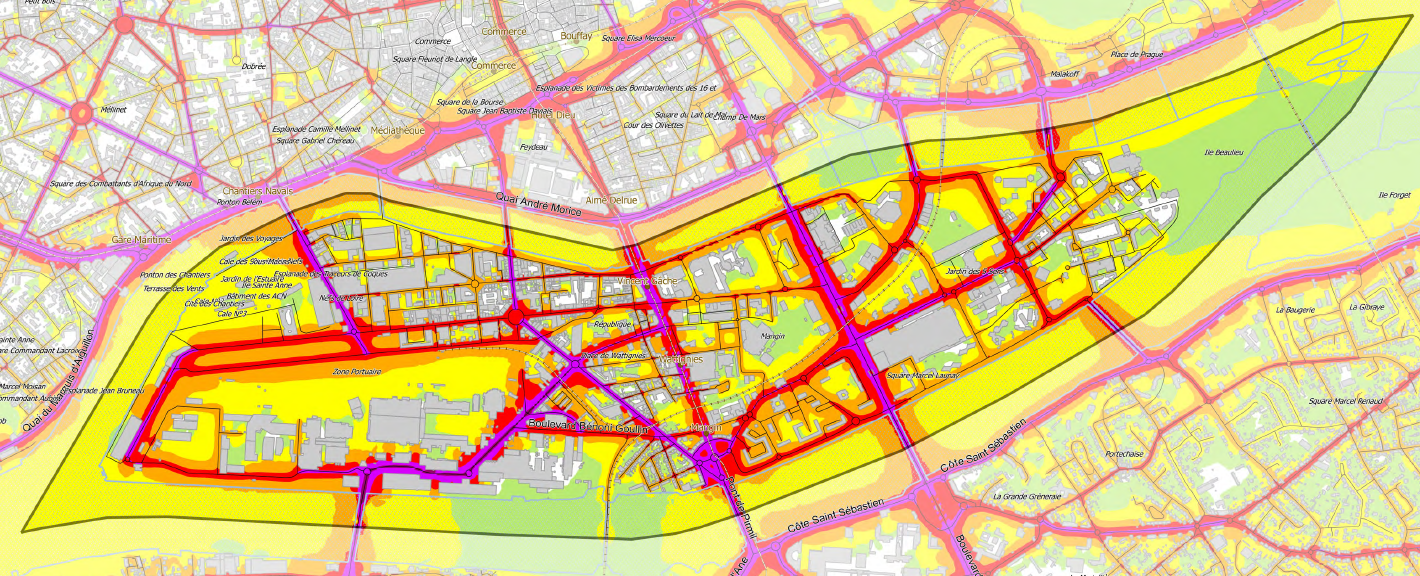
\includegraphics[scale=0.35]{./images/cartographie/Lden_ile_Nantes.PNG}}
\subfigure[]{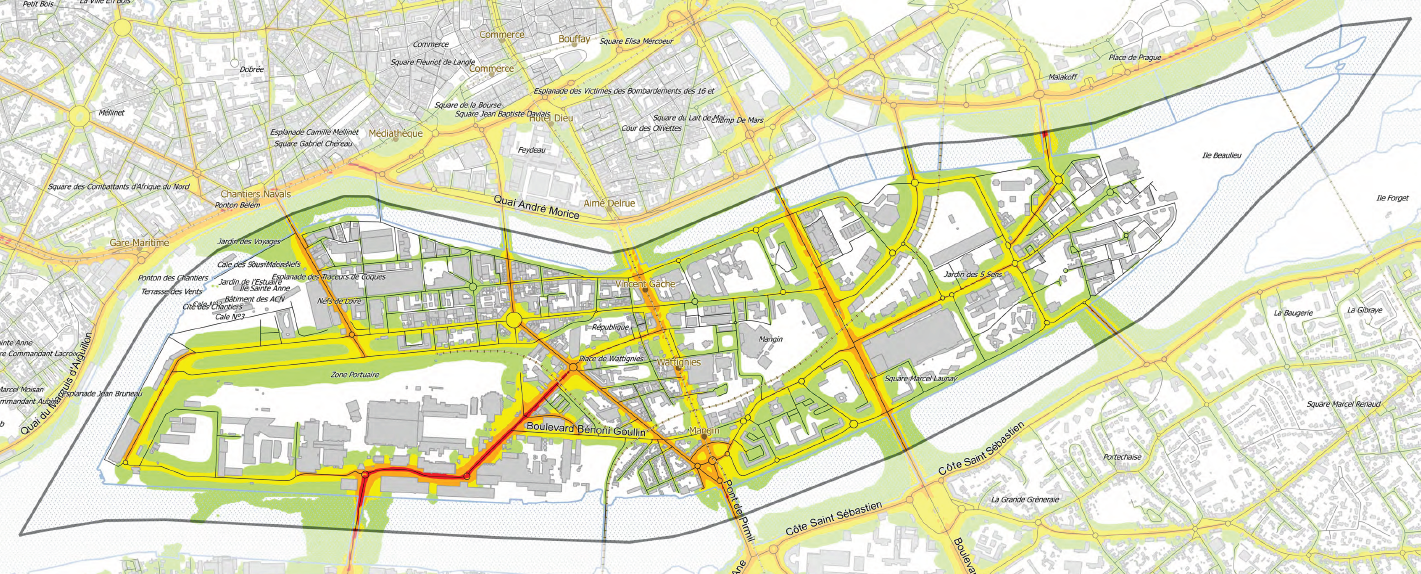
\includegraphics [scale=0.35]{./images/cartographie/Ln_ile_Nantes.PNG}}
\caption{$L_{den}$ (a) et $L_n$ (b) de l'île de Nantes pour le trafic routier \cite{nantes_carte}}
\label{fig:carto_nantes}
\end{figure}

Des données d'entrées, les niveaux sonores sont calculés à partir de modèles pré-existant(NMPB-routes-2008\cite{setra_prevision_2009-1} \cite{setra_prevision_2009-2}, CNOSSOS-EU \cite{CNOSSOS}, RSL-90 \dots). La génération des cartes se fait la plupart du temps par des bureaux acoustiques à l'aide des logiciels du commerce comme Mithra, CadnaA, Immi \dots qui font alors le choix d'utiliser un modèle de propagation parmi ceux existant. Actuellement, la méthode CNOSSOS-EU est l'approche la plus couramment utilisée à l'échelle de l'UE. Mais à l'heure actuel, ce sont les logiciel accompagné d'un Système d'Information Géographique (ou GIS pour \textit{Geographic Information System} en anglais) qui offrent le plus de possibilité. Un GIS est un système informatique conçu pour stocker, analyser et manipuler plusieurs type de données spatiales et géographiques comme l'architecture des villes ou le nombre d'habitants populations présents. Leur utilisation permettent ainsi d'améliorer la qualité des cartes et de mieux connaitre l'impact des niveaux sonores sur les citadins \cite{murphy_scenario_2011}. Par exemple, le logiciel OrbisGIS\footnote{\url{http://orbisgis.org/}}, destiné à réaliser de la représentation de données spatiales, permet la réalisation de cartes de bruit à l'aide de l'ajout d'un plugin, \textit{Noise Modelling}, développé par \cite{fortin:hal-00845701}.\\

De nombreuses études basées sur l'étude du bruit en ville ou sur la réalisation de cartes de bruit dans des quartiers utilisent comme référence cette directive \cite{murphy_environmental_2006}, \cite{murphy_estimating_2009}, \cite{Eriksson_residential_2013}. Cependant, si l'utilité de ces cartes n'est pas remis en cause, leur application ou les erreurs d'interprétations qu'elles peuvent engendrer sont toutefois questionnés.  

\section{Limites et incertitudes des cartes de bruits simulées}

L'ensemble des différentes étapes pour générer les cartes de bruits sont parfois discutées en raison des erreurs ou des incertitudes qu'elles peuvent générer. Ces erreurs sont liées aux choix de la méthode de calcul employée, aux incertitudes liées aux calculs numériques et aux indicateurs sélectionnés.

\subsection{Incertitudes liées à la méthode de calculs}

Avant même la mise en place de la directive, Steele, dans \cite{steele_critical_2001}, avait comparé les méthodes de calculs (données d'entrée, type de cartographie, méthode de propagation des différents logiciels (MITHRA, RLS90, STL-86 \dots). Parmi cette diversité d'outils, l'auteur met en avant le problème, soulevé également par \cite{king_implementation_2011}, de la diversité des outils et des méthodes de calculs que peuvent employer les professionnels. Dans \cite{garg_critical_2014}, Garg et Maji élargissent la comparaison à 8 méthodes de calcul (FHWA, CoRTN, RLS90, ASJ RTN, Harmonoise, Son Road, Nord 2000n NMPB-Routes-2008) selon de nombreux point techniques : 

\begin{itemize}
\item modélisation des sources sonores (trafic, ferroviaire), 
\item condition de trafic (constantes, accélération/décélération, intersection \dots), 
\item le modèle de propagation, 
\item la prise en compte de la divergence géométrique, 
\item les données d'entrées prise en compte, 
\item la modélisation des effets de sol,
\item les effets météorologiques,
\item les effets de diffraction,
\item \dots  \\
\end{itemize}

Par exemple, la méthode RLS-90 est la seul à prédire la densité de trafic sur les axes routier, la catégorisation des véhicules varient également entre les méthodes : dans la méthode Nord-2000 les véhicules sont divisés en 3 catégories selon leur poids alors que dans Son Road, il n'y en a que 2. Dans le cas du modèle de propagation, Harmonoise propose 3 méthodes (équation parabolique, tir de rayon et éléments de frontières) afin de s'adapter à différentes configuration là où dans FHWA c'est l'équation de propagation qui est résolue en prenant en compte des phénomènes comme l'absorption atmosphérique, les impédances des différentes surfaces rencontrées \dots Enfin les effets météorologiques sont pris en compte dans la méthodes NMPB suppose des conditions homogènes et favorable à la propagation, dans Nord 2000, le gradient e température et de vent sont inclu alors que dans les modèles Son Road et CoRTN ces phénomènes ne sont pas pris en compte. L'ensemble des nombreux points qui amènent donc des résultats divergeant entre les méthodes est alors classée en 4 catégories : émissions sonores, propagation acoustique, caractéristique de la route et autres facteurs. L'auteur conclut enfin qu'il est difficile de déterminer un \og meilleur \fg{} modèle par rapport aux autres car chacun lors de sa conception a été validé et prend en compte des phénomènes qui ne sont pas décrit par d'autres méthodes. La nécessité d'utiliser une méthode harmonisée à l'échelle européenne est ainsi proposé, par l'application de la méthode CNOSSOS-EU. 

\subsection{Incertitudes liées à la modélisation numérique}

Les cartes de bruits étant simulées, des problèmes apparaissent également lié à la modélisation et à la discrétisation du milieu urbain. Afin de limité la durée des calculs de techniques d'optimisation sont utilisées comme la discrétisation du milieu mais aussi des sources de bruits. Par exemple, pour une route décrite comme une source linéique de bruit, celle est discrétisé en un ensemble de source ponctuel alignées. Le choix de la distance entre ces points est alors un compromis à faire entre temps de calcul et précision souhaitée. Toutefois la position de ces sources influe ensuite sur les phénomènes de réflexion et de diffraction. De plus, afin de réduire les temps de calculs, les niveaux sonores entre les points calculés sont déterminés au moyen d'un calcul d'interpolation (méthode de Krigeage) qui viennent donc rajouter en plus des incertitudes \cite{van_leeuwen_noise_2015}. 

IMAGE d'INTERPOLATION ?

Enfin toujours en raison de la limitation des moyens numériques, l'effet de l'architecture urbaine (balcon, fenêtre) ou du mobilier urbain n'est pas pris en compte dans la modélisation des villes car trop complexe à réaliser alors que ces éléments ont un impact qui n'est pas pris en compte. 

\subsection{Représentation des données et estimation du nombre de citadins touché}

Une fois la carte produite, les valeurs $L_{DEN}$ et $L_N$ sont obtenues. Une critique faites de ces valeurs est la restriction d'informations qu'elles amènent. En effet, l'utilisation de ces deux valeurs pour résumer les niveaux sonores dans la ville, pendant une durée de 5 ans, est trop limitée. Tout d'abord, ces indicateurs ne donnent qu'un aperçu très générale d'une grandeur qui pourtant évolue constamment. En effet, aussi bien à l'échelle de l'année ou d'une journée, le trafic routier évolue. Cette évolution peut se diviser en 4 parties : un pic de trafic situé entre 7h et 9h et entre 16h et 18h correspondant au moment où les citadins emprunte leur voiture pour se déplacer entre leur domicile et leur travail. Entre ces 2 périodes, la quantité de voiture est plus faible \cite{}. La prise en compte ces évolutions de débit de trafic dans les modèles afin de simuler des cartes heures par heures est toutefois compliqué à mettre en oeuvre car elle nécessiterait de grande quantité de ressources informatiques et cette approche ne permettrait pas d'obtenir l'évolution annuelle. Dans \cite{modiuszeski}, Modiuszeski compare le niveau sonore simulée prédit par la carte de bruit avec les résultats de mesures réalisée toute l'année. Il constate alors aisément que l'évolution des niveaux sonores évolue autant à l'échelle de la journée que de l'année rendant les valeurs $L_{DEN}$ et $L_N$ extrêmement restrictives. Enfin, au fur et à mesure que la perception du citadin de l'environnement sonore est mieux connu, il a été montré que les indicateurs de niveaux sonores du trafic pondéré A n'est pas suffisant pour rendre compte de sa perception de l'environnement sonore. Selon, le cadre architecturale de la ville, le statu social du citadin et les sources sonores présentes, pour un niveau sonore trafic similaire, l'agrément de l'ambiance sonore par le citatdin eut ne pas être la même. En conséquence, à partir des études sur le \textit{soundscape} \cite{schafer_soundscape_1993}, il peut être envisagé de réaliser des cartes de bruits, non plus liées à une seule source de bruit, mais à la perception du citadin de l'environnement sonore (\og agréable \fg{}, \og très désagréable \fg{}, \dots). Ces cartes ne se feraient plus alors à partir d'une source de bruit mais sur l'ensemble des sources sonores présentes dans les zones et permettraient, au citadin, de savoir si tel quartier a un environnement sonore agréable ou non.\\

Des indicateurs de niveaux sonore, le nombre de citadins exposés au bruit peut être déterminé. Là encore, la méthode pour estimer ce chiffre est discutable. King et Murphy résument cela dans un paragraphe dans \cite{king_implementation_2011}. L'hypothèse faite est que les individus vivent et dorment toute l'année au niveau de la façade la plus exposée, ce qui n'est pas forcément représentatif de la réalité. Cette hypothèse conduit notamment à une surestimation du nombre de personnes touché par des niveaux sonores. \\

La réalisation de ces cartes visant à diminuer l'exposition des citadins au forts niveaux sonores, les incertitudes provoquées par les différents étapes peuvent entrainer la mise en chantier d'un plan d'action mal adapté à la situation réelle. Mais l'amélioration des cartes, telles qu'elles sont faites actuellement, semble toutefois limité : l'augmentation de la résolution des permettrait bien de corriger certaines erreurs dû aux interpolations mais viendrait à augmenter considérablement les cout de calculs. De plus, ce choix rendrait impossible de mettre à jours les cartes régulièrement pour prendre en compte les fluctuations du trafic à l'échelle de l'année ou même encore durant la journée. En conséquence, à l'heure où les villes s'équipent en réseaux de capteurs (météorologique, pollution) en vue de devenir des \og villes intelligentes \fg{} (\textit{smart cities} en anglais), plusieurs recherches se proposent d'y ajouter des capteurs acoustiques afin de s'en servir pour la cartographie du bruit de trafic les cartes simulées. \\


\section{Utilité de l'apport de mesures}

L'intérêt de l'utilisation de mesures faites directement en ville est qu'elles rendent possible d'obtenir des informations sur les niveaux sonores des sources présente directement dans les rues et non plus par simulation. \`A partir des mesures, en sachant estimer le niveau sonore du trafic routier, aérien, ferroviaire et des industries, il serait envisageable de réaliser des cartes de bruit dynamiques, c'est-à-dire mises à jours régulièrement (tous les jours ou toutes les heures) \cite{wei_monitoring_2014} ou bien encore d'ajuster les cartes pré-existantes \cite{makarewicz_empirical_2011}. Plusieurs approches sont envisagées pour réaliser cela aux travers de mesures mobiles \cite{can_exploring_2012} ou fixes \cite{zannin_characterization_2013}.


\subsection{Utilisation des réseaux de capteurs}

Grâce à l'évolution des moyens de communication et au développement de capteurs à bas coûts, une des pistes envisagées est l'utilisation de réseaux de capteurs qui sont actuellement déployé dans certaines villes d'Europe. Cette approche consiste à installer dans un quartier un ensemble de microphones qui vont réaliser des enregistrements et des mesures. 

CARTE AVEC RESEAUX MICROPHONES (CENSE)

Ces réseaux, couplés à des méthodes de détection et de reconnaissance de sources, trouvent plusieurs applications notamment auprès de la sécurité et de la surveillance \cite{simon_sensor_2004} \cite{foggia_audio_2016}. Dans le cadre de l'amélioration de la cartographie du bruit de trafic, ces réseaux permettraient d'avoir une mesure \textit{in situ} du trafic. \`A l'heure actuel, plusieurs projets étudient la mise en place et la faisabilité de telle installations comme le projet italien DYNAMAP \cite{dynamap_2016}. Ce projet a pour objectif de développer un système de cartographie de bruit dynamique basé sur des réseaux de capteurs à bas coûts installés en ville. Une application de ce projet a déjà été réalisé dans deux villes tests, Milan et Rome \cite{bellucci_life_2017}. 

En Chine, on peut relever l'expérimentation de Cai $\&$ al. \cite{cai_road_2014}  qui a comparer les résultats obtenu par un logiciel GIS avec un réseau de microphone. 
En France, le projet RUMEUR \cite{mietlicki2012innovative} en région parisienne existe déjà depuis plusieurs années et a consisté à déployer des réseaux de microphones destiné à la mesure du bruit aérien. Un site internet\footnote{\url{http://rumeur.bruitparif.fr/}} permet alors au citoyen d'avoir un aperçu complet des mesures réalisées sur de nombreux sites et de voir l'impact de bruit aérien dans ces zones. Enfin, le projet CENSE\footnote{\url{http://cense.ifsttar.fr/}} vise à développer un outil permettant d'agréger les données simulées du niveaux sonores du trafic avec des mesures réalisées en villes par des réseaux de capteurs. De plus, les aspects perceptifs et \textit{soundscape} sont également étudiés en vue de d'obtenir une caracétérisation plus fine de l'environnement sonore urbain (\cite{can_describing_2015}, \cite{brocolini_measurements_2013}). Une des difficultés quant à l'utilisation de réseaux de capteurs fixes est celle de de la spatialisation des mesures et de la surface couverte par ces mesures : un réseau distribué selon un maillage dense permettra une bonne représentation de l'espace mais coutera cher à installer et à maintenir alors qu'une faible densité de capteur apportera peu d'information et nécessitera des interpolations entre les mesures, sources d'incertitudes. Dans le projet DYNAMAP, les stations fixes sont installées à des endroits représentatifs des différents scénarios routier possible sur l'ensemble de la ville (trafic homogène, type de surface, type de trafic\dots) alors que dans CENSE les capteurs sont situés à l'échelle d'un quartier. Différentes méthodes d'interpolations existent alors pour pouvoir estimer les niveaux sonores dans les zones non couvertes (méthode krigeage,  \\

\subsection{Mesures mobiles}
En parallèle, la mesure mobile est une approche qui est elle aussi permettre l'amélioration de la cartographie de bruit de trafic. Elle consiste à réaliser des mesures en plaçant le microphone sur un support en mouvement (piéton, cycliste, voiture, bus). L'avantage de cette méthode est sa capacité à pouvoir couvrir plus facilement une plus grande surface urbaine à moindre coût. Les mesures mobiles sous-entendent deux manières d'être réalisées : soit la mesure est réalisé alors que son support bouge \cite{alsina-pages_design_2016} et dans ce cas un traitement du signal doit être effectué pour prendre en compte le bruit émis par ce support, soit le support permet de déplacer le microphone pour faire ensuite des mesures fixes \cite{manvell_sadman_2004} ce qui permet de simplifier la tâche mais qui nécessite plus de temps pour couvrir une surface similaire aux mesures faites sur supports mobiles. 

Le problème reste celui de la spatialisation et de l'interpolation des mesures. Dans \cite{can_measurement_2014}, à partir de mesures fixes, 2 méthodes classiques d'interpolations (méthode de distance pondérée inverse et méthode de Krigeage) sont testées et comparées à l'interpolation produite avec des mesures mobiles. Il en résulte que l'apport des mesures mobiles diminue l'erreur produite par rapport aux méthodes d'interpolation en cela qu'elles permettent d'apporter beaucoup d'informations quant aux variations spatiales du niveau sonore (rues calmes peu fréquentées, rue très passante)et aux variations spatiales provoquées par le trafic (intersection, tramway, rues piétonnes \dots) ce que ne permet pas une méthode d'interpolation numérique.

\subsection{Mesures participatives}
Enfin, dans le but de toujours plus sensibiliser le citadin à son environnement sonore, leur participation est sollicité. Celle-ci peut être sollicité soit à travers des campagnes de mesures où des dispositifs professionnels leur est donné \cite{} ou bien à travers leur propre-chef en utilisation des applications développées pour smartphones, comme  que des citadins pourront alors utilisés. Profitant de la démocratisation de ces appareils et de l'augmentation de leur performances, ces applications leur permet d'avoir l'équivalent d'un sonomètre dans leur poche. L'utilisation de ces mesures est toutefois encore sujet à caution puisque de nombreux problèmes sont à résoudre : calibration et performances des microphones dans les faibles et forts niveaux sonores, qualité de la réalisation de la mesure par l'utilisateur \dots Cette approche permet surtout d'obtenir un plus grand nombre de mesures qui ont le plus souvent une distribution spatiale plus aléatoire mais qui sont aussi moins effectuées régulièrement. Dans ce cas, le traitement statistique des résultats est un enjeu majeur afin de pouvoir utiliser correctement les résultats de ces mesures \cite{guillaume2016noise}. Plusieurs projets ont été réalisés comme l'outil  NoiseSpy \cite{kanjo_noisespy_2010}. Dans son article, Kanjo détaille les


On peut également relever le projet \textit{Noise Planet}\footnote{\url{http://noise-planet.org}} qui a pour objectif de proposer un outil libre et gratuit pour évaluer le bruit de l'environnement sonore. Il comprend un application pour smartphone, NoiseCapture \cite{guillaume2016noise}, qui permet là encore à l'utilisateur d'évaluer les niveaux sonores l'entourant tout en ayant la possibilité de décrire à l'aide mots-clés prédéfini les sons présents et l'ambiance sonore de la scène. 

\begin{figure}
\begin{center}
    \begin{minipage}[t]{0.3\textwidth}
        \centering
        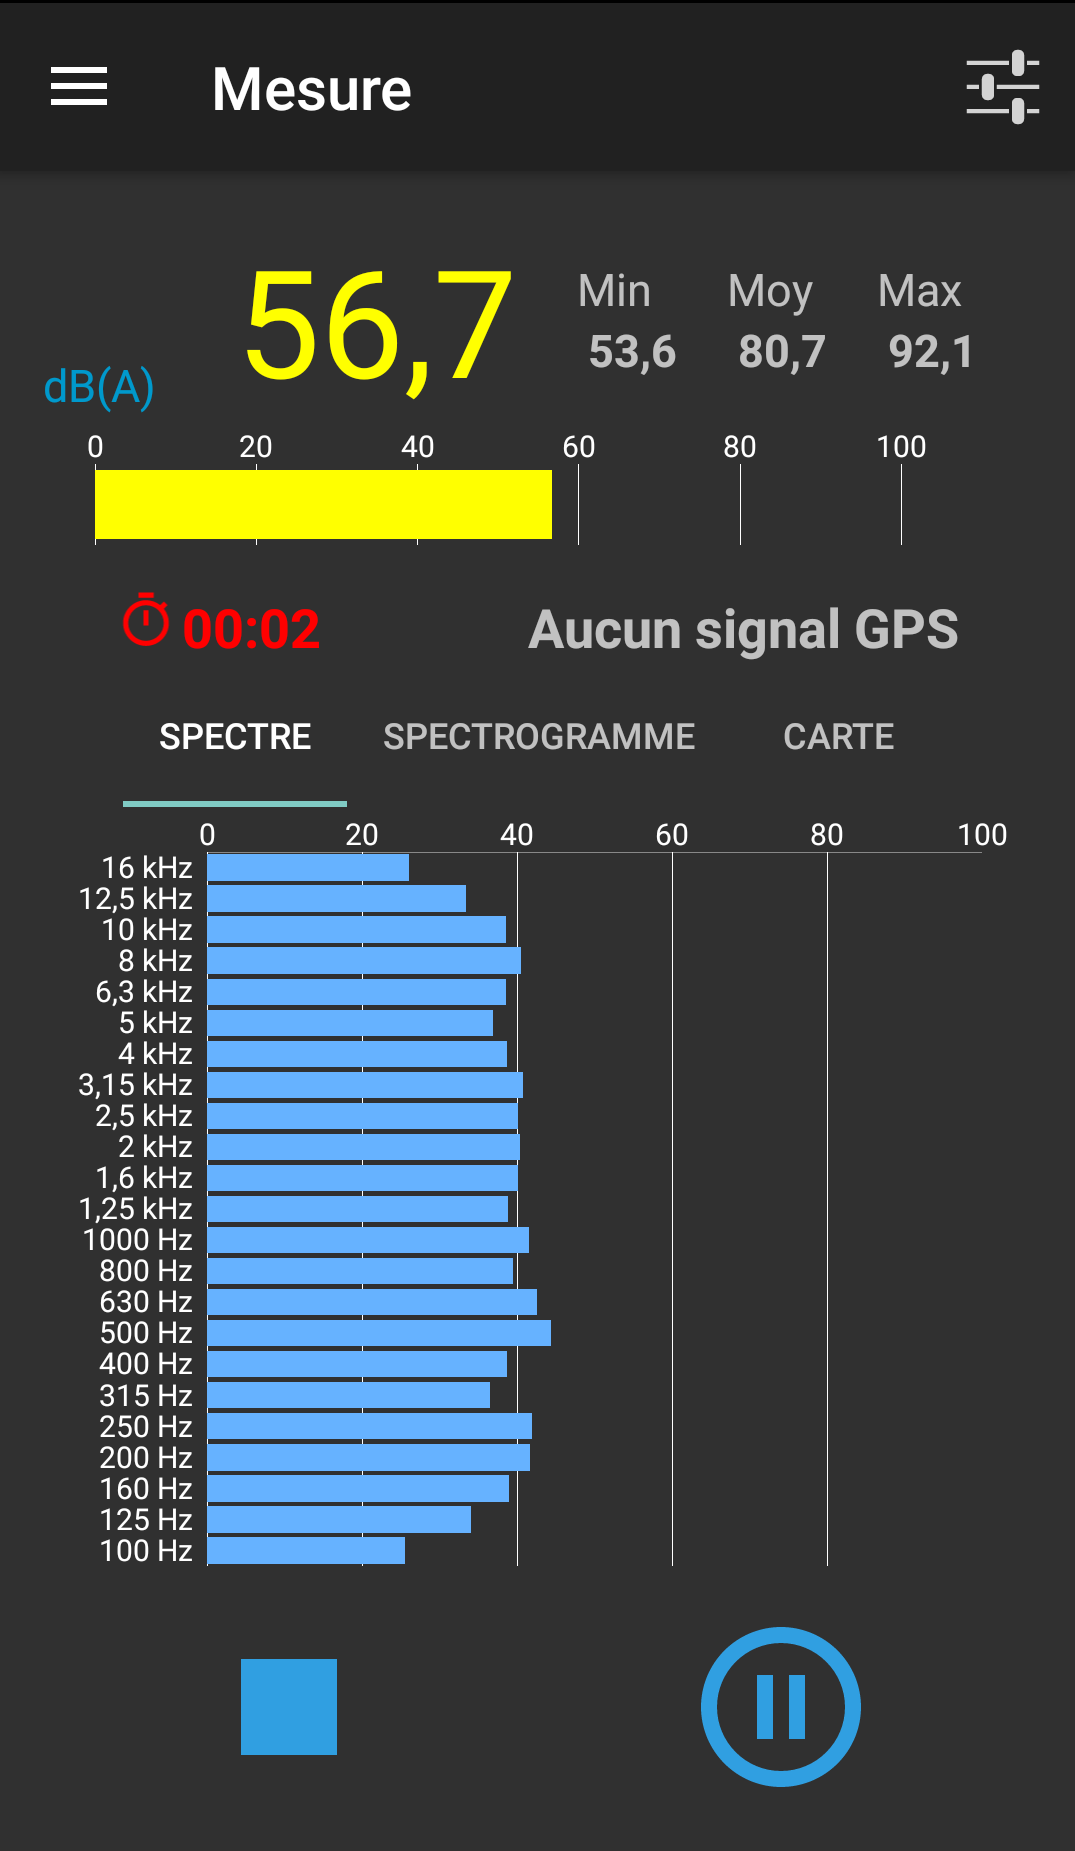
\includegraphics[width=0.9\textwidth]{../../../Pictures/autres/noiseCapture1.png}
    \end{minipage}
    \begin{minipage}[t]{0.3\textwidth}
        \centering
        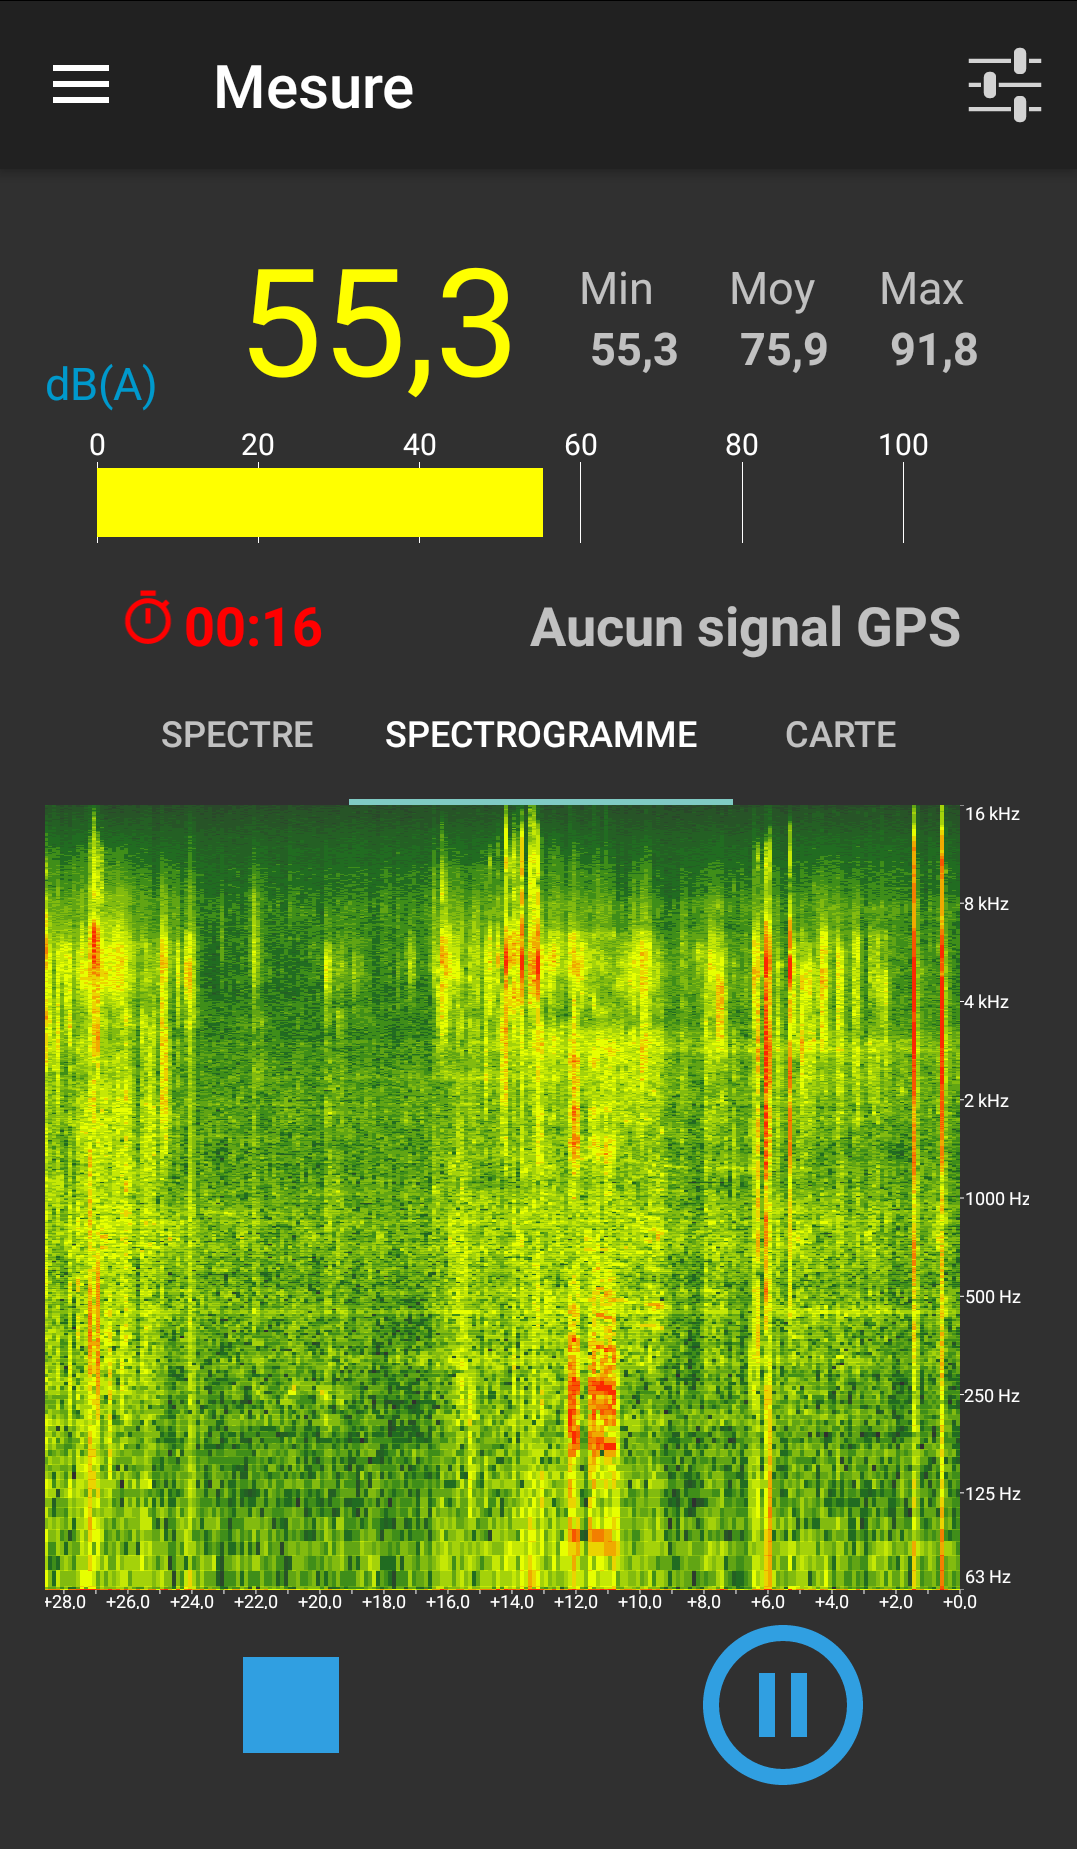
\includegraphics[width=0.9\textwidth]{../../../Pictures/autres/noiseCapture3.png}
    \end{minipage}
    \begin{minipage}[t]{0.3\textwidth}
        \centering
        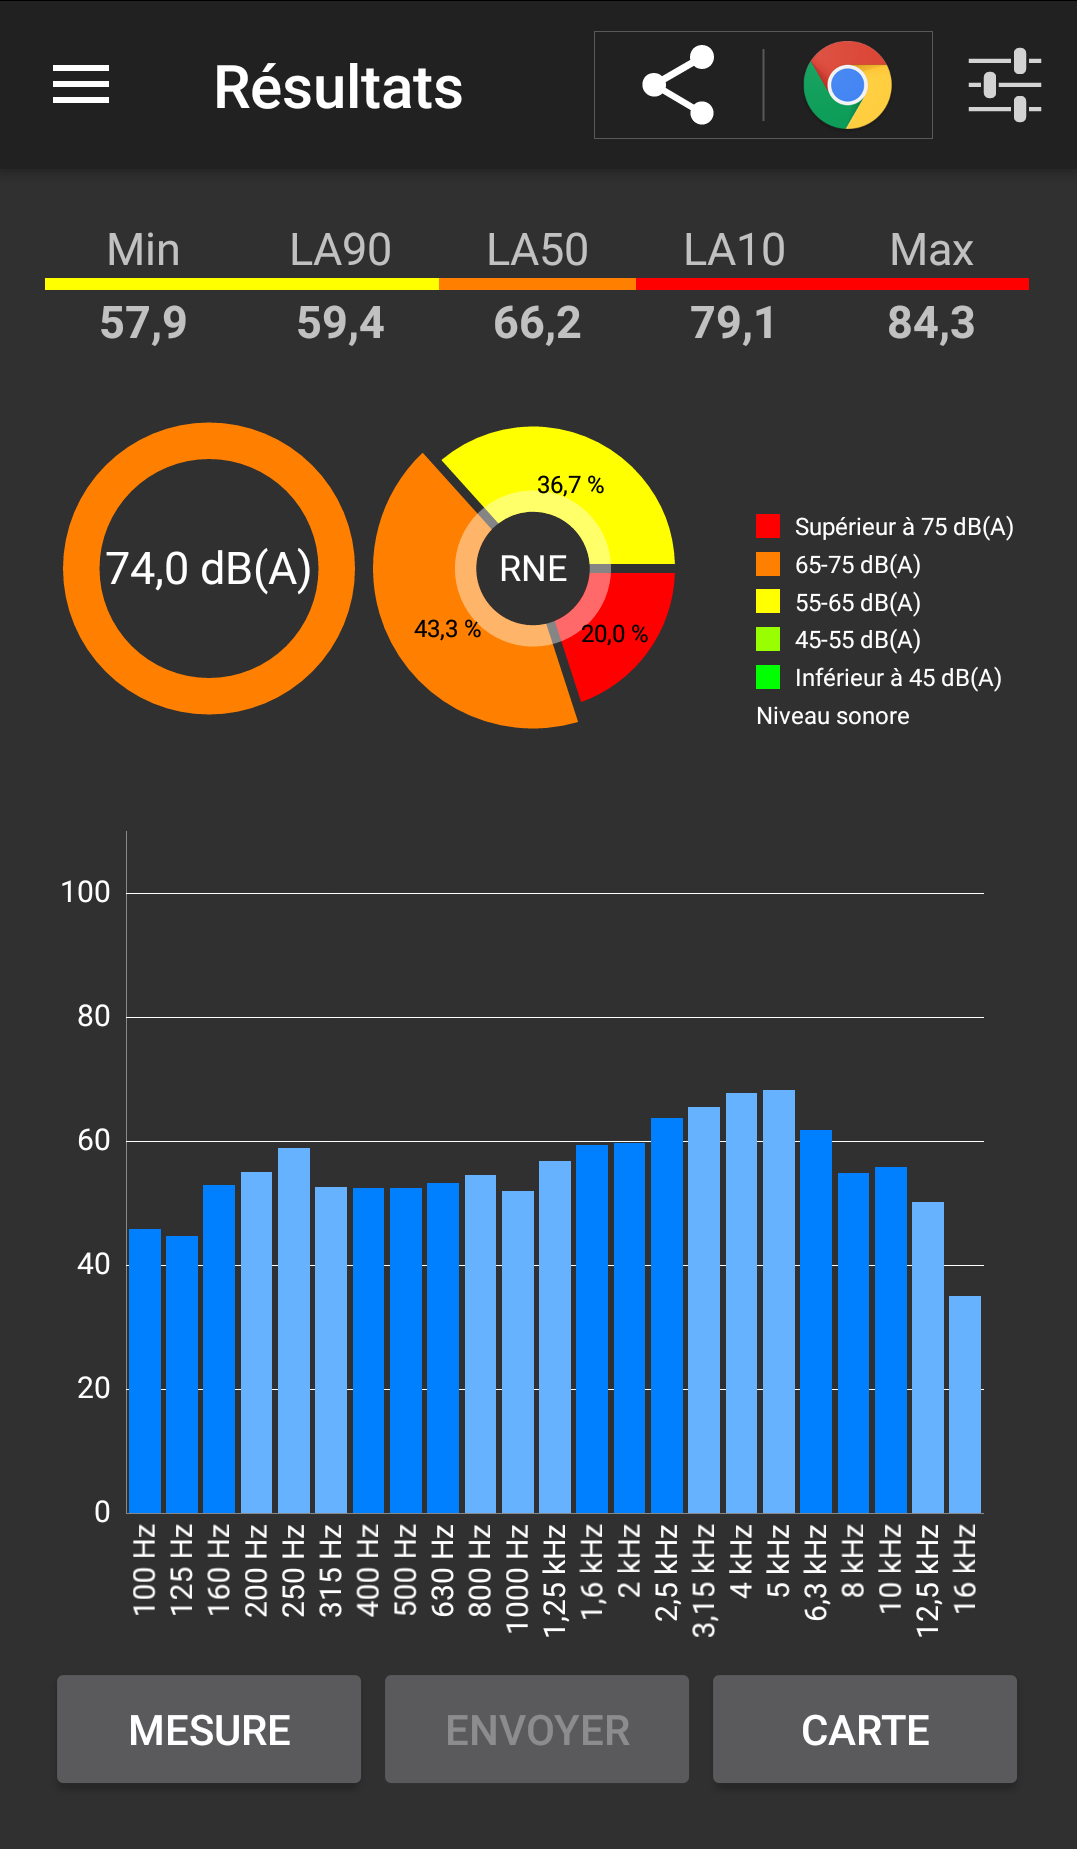
\includegraphics[width=0.9\textwidth]{../../../Pictures/autres/noiseCapture2.png}
    \end{minipage}
    \caption{Captures d'écran de l'application \textit{NoiseCapture}}
\end{center}
\end{figure}


La géo-localisation et les mesures sont ensuites collectées puis traitées par le système OnoM@p \cite{bocher_onomp_2016}. Puis dans une troisième étape, l'outil \textit{Noise Modelling} permet, à partir de ces mesures, sous le logiciel OrbisGIS, de générer des cartes de bruits, publiées en ligne.\\

Toutefois, malgré ces différentes approches composés de mesures acoustique, en vue d'améliorer la cartographie de bruit de trafic, la question de l'estimation du niveau sonore du trafic reste posée et peut se révéler délicate à répondre. En effet, en ville, il existe de nombreuses sources sonores qui s'ajoutent au trafic : musique, bruit de pas et de conversations, sirènes, aboiement, sifflement d'oiseaux ... Ce sont donc de nombreuses sources ayant leurs propres évolutions temporelles et fréquentielles qui viennent s'ajouter à celui du trafic. Dans son article Mioduszewski reconnait ce problème sans toutefois le corriger \cite{Mioduszewski}.\\

La prise en compte quelconque de toute les sources sonores présentes dans les mesures, dans certains cas, engendre indubitablement une surestimation du niveau sonore du trafic qui viendrait alors fausser les cartes de bruits. Il est donc nécessaire de savoir isoler les éléments relatifs au trafic des autres sources sonores dans les mesures réalisées afin de mieux estimer leur niveaux sonores. La création d'un tel outil présenterait des avantages notables : puisqu'il est possible de déterminer la contribution du bruit du trafic, il est envisageable d'extraire également d'autres type de bruit comme les sifflements des oiseaux, le brouhaha de la rue ou d'une cours de récréation... Ces sources sonores isolées mènerait ainsi à la formation de cartes ciblées sur certains types de bruit et pouvant mener à la création de cartes d'agréments sonores. Enfin, il serait alors possible de comparer les résultats expérimentaux et simulés en ne tenant compte réellement que de la contribution du trafic routier.

%\bibliographystyle{unsrt}
%\bibliography{../bibliographie}
%
%\end{document} 